\section{Evaluation}


\subsection{Environment and Setup}

\noindent\textbf{Cloud deployment.}
All experiments run on Amazon Web Services (AWS). Single-node experiments use one r6a.32xlarge EC2 instance with 128 vCPUs and 1~TB of memory. Distributed experiments use up to ten m6a.4xlarge instances, each with 16 vCPUs and 64~GB of memory. The orchestrator runs on one worker instance, so all instances remain available for proving.

\noindent\textbf{Baselines.}
Our primary baseline is monolithic EZKL, which compiles and proves the full model as a single circuit on one machine. We compare it with EZKL+\TITLE{}, which uses the same proving backend but partitions execution into proving jobs. We also evaluate zkTorch~\cite{chen2025zktorch} with and without \TITLE{} to test portability across zkML backends.

\noindent\textbf{Workloads.}
Table~\ref{tab:models} summarizes the evaluation workloads, spanning convolutional vision, image generation, and transformer models with different circuit sizes and partitioning structures. The two NanoGPT configurations additionally vary model depth while holding architecture family and sequence length fixed.

\noindent\textbf{Measurement methodology.}
Unless otherwise stated, results are averaged over three runs. End-to-end latency is measured from request submission until the model output and all job-level proofs are available. For \TITLE{}, this includes partitioning, boundary-tensor materialization, artifact lookup or generation, scheduling, and proof generation, but excludes client-side verification.



\begin{table*}[t]
\centering
\renewcommand{\arraystretch}{1.05}
\setlength{\tabcolsep}{5pt}

\newcommand{\upchange}[1]{\textcolor{gray}{\scriptsize $\uparrow #1\times$}}
\newcommand{\downchange}[1]{\textcolor{gray}{\scriptsize $\downarrow #1\times$}}
\newcommand{\metric}[2]{\makecell[c]{#1\\[-2pt]#2}}

\begin{tabular*}{\textwidth}{@{\extracolsep{\fill}} l l c c c c}
\toprule
\textbf{Model} &
\textbf{System} &
\textbf{Constraints (M)} &
\textbf{PK Storage (GB)} &
\textbf{Cold E2E (s)} &
\textbf{Warm E2E (s)} \\
\midrule

MobileNetV2
  & EZKL
  & 67.10
  & 312.31
  & \num{25652}
  & \num{11231} \\
  & \TITLE{}+EZKL
  & \metric{94.43}{\upchange{1.41}}
  & \metric{271.99}{\downchange{1.15}}
  & \metric{\num{16050}}{\downchange{1.6}}
  & \metric{\num{9639}}{\downchange{1.2}} \\
\midrule

NanoGPT (4L)
  & EZKL
  & 16.77
  & 262.14
  & \num{8527}
  & \num{6165} \\
  & \TITLE{}+EZKL
  & \metric{18.03}{\upchange{1.08}}
  & \metric{59.33}{\downchange{4.42}}
  & \metric{\num{2520}}{\downchange{3.4}}
  & \metric{\num{1108}}{\downchange{5.6}} \\
\midrule

NanoGPT (10L)
  & EZKL
  & OOM
  & OOM
  & OOM
  & OOM \\
  & \TITLE{}+EZKL
  & 29.15
  & 146.88
  & \num{8066}
  & \num{2683} \\
\midrule

MNIST-GAN Gen.
  & EZKL
  & 8.38
  & 43.52
  & \num{2352}
  & \num{808} \\
  & \TITLE{}+EZKL
  & \metric{9.56}{\upchange{1.14}}
  & \metric{47.52}{\upchange{1.09}}
  & \metric{\num{1852}}{\downchange{1.3}}
  & \metric{\num{456}}{\downchange{1.8}} \\
\midrule

TinyBERT
  & EZKL
  & 8.38
  & 131.07
  & \num{4539}
  & \num{2194} \\
  & \TITLE{}+EZKL
  & \metric{18.63}{\upchange{2.22}}
  & \metric{68.98}{\downchange{1.90}}
  & \metric{\num{2700}}{\downchange{1.7}}
  & \metric{\num{1022}}{\downchange{2.1}} \\

\bottomrule
\end{tabular*}

\caption{
Single-worker end-to-end performance for EZKL and \TITLE{}+EZKL.
Cold requests generate setup artifacts; warm requests reuse them.
Small values report change relative to EZKL; OOM denotes out-of-memory.
}
\label{tab:splitting-results}
\end{table*}








% \begin{table*}[tb]
% \small
% \centering
% \setlength{\tabcolsep}{4.5pt}
% \renewcommand{\arraystretch}{0.88}


% \begin{tabular*}{\textwidth}{@{\extracolsep{\fill}} l l c c c c}
% \toprule
% \textbf{Model} &
% \textbf{System} &
% \textbf{Constraints (M)} &
% \textbf{PK Storage (GB)} &
% \textbf{Cold E2E (s)} &
% \textbf{Warm E2E (s)} \\
% \midrule

% MobileNetV2
%   & EZKL            & 67.10 & 312.31 & \num{25652} & \num{11231} \\
%   & \TITLE{}+EZKL   & 94.43 (\(\uparrow 1.41\times\)) & 271.99 (\(\downarrow 1.15\times\)) & \num{16050} (\(\downarrow 1.6\times\)) & \num{9639} (\(\downarrow 1.2\times\)) \\
% \midrule

% NanoGPT (4L)
%   & EZKL            & 16.77 & 262.14 & \num{8527}  & \num{6165} \\
%   & \TITLE{}+EZKL   & 18.03 (\(\uparrow 1.08\times\)) & 59.33 (\(\downarrow 4.42\times\)) & \num{2520} (\(\downarrow 3.4\times\)) & \num{1108} (\(\downarrow 5.6\times\)) \\
% \midrule

% NanoGPT (10L)
%   & EZKL            & OOM   & OOM    & OOM         & OOM \\
%   & \TITLE{}+EZKL   & 29.15 & 146.88 & \num{8066}  & \num{2683} \\
% \midrule

% MNIST-GAN Gen.
%   & EZKL            & 8.38  & 43.52  & \num{2352}  & \num{808} \\
%   & \TITLE{}+EZKL   & 9.56 (\(\uparrow 1.14\times\)) & 47.52 (\(\uparrow 1.09\times\)) & \num{1852} (\(\downarrow 1.3\times\)) & \num{456} (\(\downarrow 1.8\times\)) \\
% \midrule

% TinyBERT
%   & EZKL            & 8.38  & 131.07 & \num{4539}  & \num{2194} \\
%   & \TITLE{}+EZKL   & 18.63 (\(\uparrow 2.22\times\)) & 68.98 (\(\downarrow 1.90\times\)) & \num{2700} (\(\downarrow 1.7\times\)) & \num{1022} (\(\downarrow 2.1\times\)) \\

% \bottomrule
% \end{tabular*}

% \caption{
% Single-worker end-to-end performance for monolithic EZKL and \TITLE{}+EZKL.
% Cold requests do not assume cached proving artifacts, while warm requests reuse cached artifacts.
% Parentheses report the relative change compared with EZKL; OOM indicates that the monolithic baseline ran out of memory.
% }
% \label{tab:splitting-results}
% \end{table*}





% \begin{table}[t]
% \small
% \centering
% \setlength{\tabcolsep}{4pt}
% \begin{tabular}{l r r r}
% \toprule
% \textbf{Model} &
% \makecell{\textbf{EZKL}\\\textbf{mono}} &
% \makecell{\textbf{\TITLE{}}\\\textbf{1W}} &
% \makecell{\textbf{\TITLE{}}\\\textbf{15W}} \\
% \midrule
% NanoGPT (4L) & 6165s  & 1108s & 399s  \\
% MobileNetV2  & 11231s & 9639s & 2384s \\
% TinyBERT     & 2194s  & 1022s & 333s  \\
% \bottomrule
% \end{tabular}
% \caption{
% Single-node end-to-end proof-generation time. 
% \TITLE{} reduces latency even with one worker through partitioning, and further improves performance with 15 concurrent prover workers.
% }
% \label{tab:single-node-raw}
% \end{table}


% \begin{figure}[t]
% \centering
% 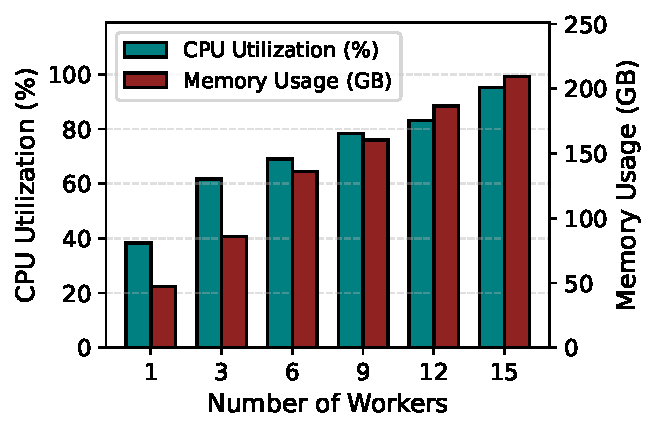
\includegraphics[width=\linewidth]{figures/evaluation/single_node_resource_usage_mobilenet_bar.pdf}
% \caption{
% Single-node resource utilization for MobileNetV2 as the number of prover workers increases. 
% Higher worker counts increase CPU and memory pressure, helping explain the sublinear scaling observed on a single machine.
% }
% \label{fig:single-node-resource}
% \end{figure}


\subsection{Monolithic vs. Partitioned Proving}
\label{sec:eval-monolithic-vs-partitioned}

We first isolate the effect of partitioning without parallel or distributed execution. Monolithic EZKL proves the full model as one circuit, while EZKL+\TITLE{} executes partitioned proving jobs sequentially on a single worker. Differences therefore reflect proving granularity rather than additional compute capacity.

Table~\ref{tab:splitting-results} reports cold and warm end-to-end latency, total constraints, and aggregate proving-key storage. Cold requests generate reusable setup artifacts, while warm requests reuse them. For EZKL+\TITLE{}, constraints and proving-key storage are summed across all jobs.

\subsubsection{\textbf{End-to-End Latency and Proving-Key Footprint}}

As shown in Table~\ref{tab:splitting-results}, \TITLE{}+EZKL is \(1.3\times\) to \(3.4\times\) faster than monolithic EZKL for cold requests and \(1.2\times\) to \(5.6\times\) faster for warm requests across the four models completed by both systems. These gains occur despite higher aggregate constraint counts, showing that proving cost depends not only on the total number of constraints but also on how they are partitioned across circuits.

\TITLE{} also reduces aggregate proving-key storage for three of the four comparable models. NanoGPT (4L) drops from 262~GB to 59~GB, while MNIST-GAN Gen.\ increases slightly from 44~GB to 48~GB. Partitioning also improves feasibility: monolithic EZKL runs out of memory on NanoGPT (10L), whereas \TITLE{}+EZKL completes it with a peak memory footprint of 11.9~GB.


\begin{figure*}[t]
\centering
\begin{subfigure}[t]{0.48\textwidth}
    \centering
    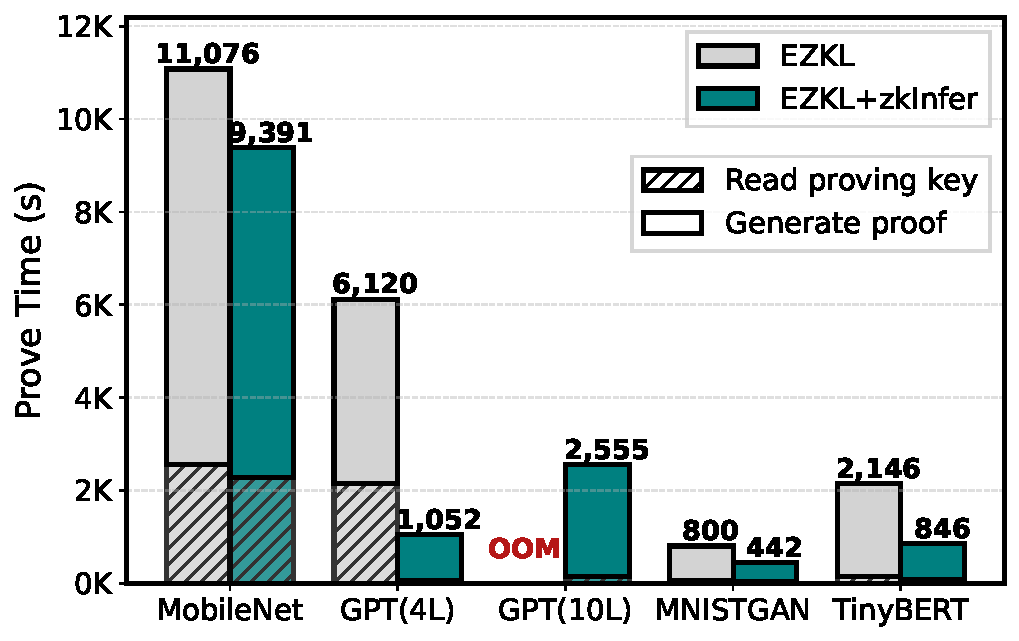
\includegraphics[width=\linewidth]{figures/evaluation/prove_time.pdf}
    \caption{Proof generation time}
    \label{fig:runtime_a}
\end{subfigure}
\hfill
\begin{subfigure}[t]{0.48\textwidth}
    \centering
    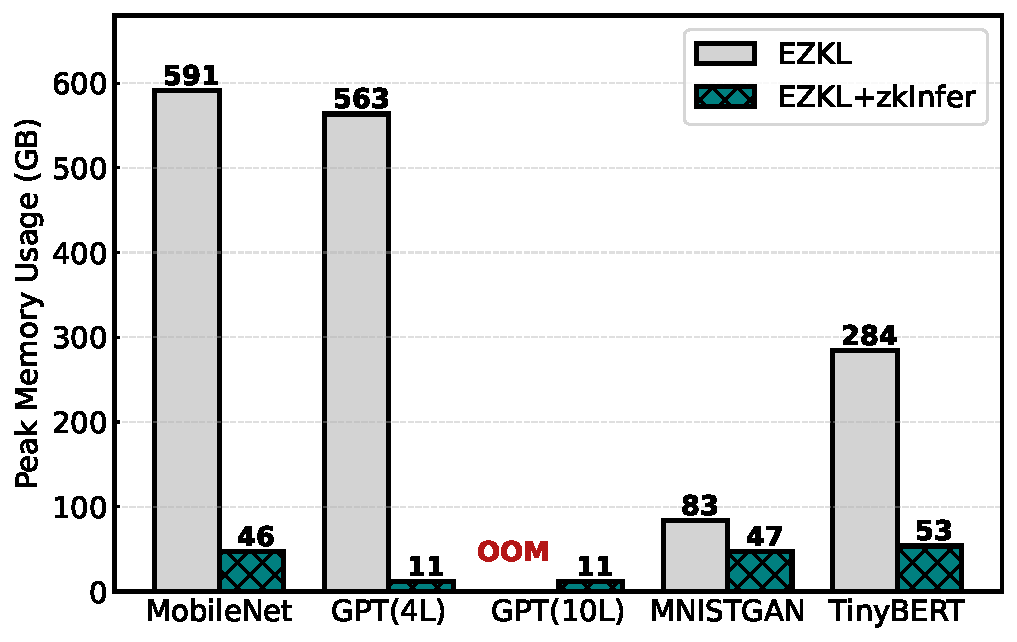
\includegraphics[width=\linewidth]{figures/evaluation/max_memory.pdf}
    \caption{Peak memory usage}
    \label{fig:runtime_memory}
\end{subfigure}
\caption{
Single-worker proof-generation performance under cached setup. 
The left plot breaks down the time required to load proving keys and generate proofs, while the right plot reports peak memory usage during proof generation. 
By reducing the size of the largest circuit instance, \TITLE{} lowers both proof-generation time and peak memory demand.
}
\label{fig:runtime_comparison}
\end{figure*}


\begin{figure*}[t]
\begin{subfigure}[t]{0.32\textwidth}
    \centering
    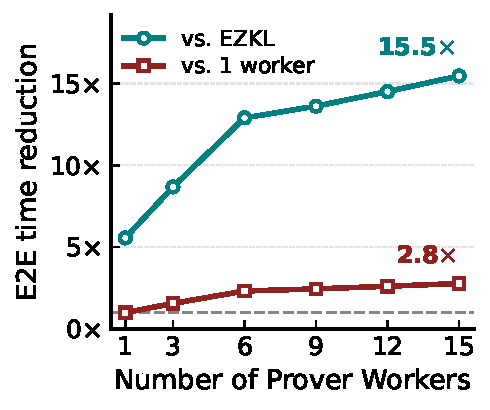
\includegraphics[width=\linewidth]{figures/new_eval/single_node_scaling_GPT_4L__time_reduction.pdf}
    \caption{NanoGPT (4L)}
    \label{fig:runtime_nano4l}
\end{subfigure}
\hfill
\begin{subfigure}[t]{0.32\textwidth}
    \centering
    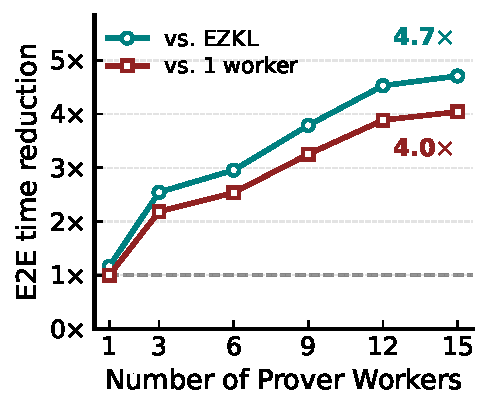
\includegraphics[width=\linewidth]{figures/new_eval/single_node_scaling_MobileNet_time_reduction.pdf}
    \caption{MobileNetV2}
    \label{fig:runtime_model2}
\end{subfigure}
\hfill
\begin{subfigure}[t]{0.32\textwidth}
    \centering
    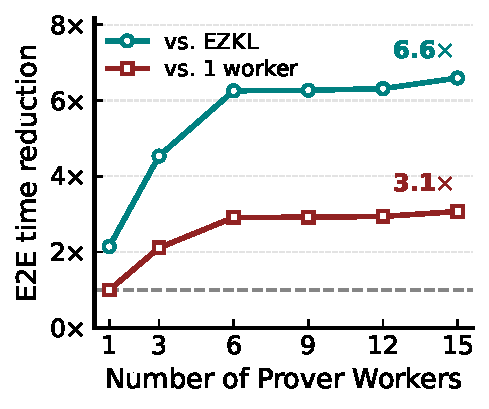
\includegraphics[width=\linewidth]{figures/new_eval/single_node_scaling_BERT_Tiny_time_reduction.pdf}
    \caption{TinyBERT}
    \label{fig:runtime_model3}
\end{subfigure}

\caption{
Single-node scaling of \TITLE{} as the number of prover workers increases. 
Each plot reports the speedup in end-to-end request time relative to the monolithic EZKL baseline and the single-worker \TITLE{}+EZKL configuration. 
}
\label{fig:parallel_single_node}
\end{figure*}

% \subsubsection{\textbf{End-to-End Serving Latency and Artifact Footprint}}
% End-to-end serving latency measures the wall-clock time from request submission until the model output and all proof material for the inference are available. For \TITLE{}, this includes model splitting, artifact lookup or generation, scheduling, and the execution of all submodel-level proving jobs. In the cold setting, \TITLE{}+EZKL improves request time for every model that completes under both systems. Speedups range from \(1.3\times\) on MNIST-GAN Gen.\ to \(3.4\times\) on NanoGPT (4L), with a geometric mean improvement of \(1.84\times\). These improvements hold even when partitioning increases the aggregate constraint count, as in MobileNetV2 and TinyBERT. This result shows that total constraint count alone is not a reliable predictor of prover performance. The size of each circuit instance also matters. By reducing the largest prover invocations, \TITLE{} lowers per-job memory pressure and execution cost enough to offset the overhead introduced by partition boundaries.

% Proving-key storage affects whether warm-request performance is practical in steady-state serving. Since proving keys are large, a system can only benefit from caching when the artifacts needed by future requests fit within the available storage budget. \TITLE{} reduces aggregate proving-key storage for several models, most notably NanoGPT (4L), where storage drops from 262~GB to 59~GB. TinyBERT and MobileNetV2 also see reductions, from 131~GB to 69~GB and from 312~GB to 272~GB, respectively. These reductions increase the likelihood that proving artifacts remain cached across repeated requests and across multiple deployed models. MNIST-GAN Gen.\ is the exception, with proving-key storage increasing slightly from 44~GB to 48~GB, reflecting its smaller number of partitions and more limited opportunity to reduce setup footprint.

% NanoGPT (10L) demonstrates the feasibility benefit of partitioned proving. The monolithic EZKL baseline runs out of memory before completing the proof, while \TITLE{}+EZKL completes the same inference request in \num{8066}s cold and \num{2683}s warm. This  shows that partitioning can reduce peak memory demand enough to make larger proving workloads tractable.

\subsubsection{\textbf{Impact on Online Proving Performance}}

We next examine the work that must be repeated for every request after
setup artifacts have been generated. At this stage, the prover must
still load the required proving keys and generate the proofs. We define
\emph{online proving time} as the sum of these two components, which
Figure~\ref{fig:runtime_a} reports separately. Across the four models that complete under both systems, \TITLE{}+EZKL
reduces online proving time by \(\num{1.2}\times\) to
\(\num{5.8}\times\). NanoGPT (4L) shows the largest improvement and
provides the clearest breakdown. Proving-key loading decreases from
\(\qty{2146}{\second}\) to \(\qty{65}{\second}\), a \(\num{33}\times\)
reduction, while proof generation decreases from \(\qty{3975}{\second}\)
to \(\qty{987}{\second}\), a \(\num{4.0}\times\) reduction. Key loading
improves disproportionately because the monolithic prover must load one
massive proving key before any work begins, whereas each partitioned job
loads only the small key it needs. Partitioning has an even larger effect on peak memory. As shown in
Figure~\ref{fig:runtime_memory}, monolithic EZKL requires
\(\qty{591}{\giga\byte}\) for MobileNetV2, \(\qty{563}{\giga\byte}\) for
NanoGPT (4L), and \(\qty{284}{\giga\byte}\) for TinyBERT. With
\TITLE{}, peak memory decreases to \(\qty{46.7}{\giga\byte}\),
\(\qty{11.6}{\giga\byte}\), and \(\qty{53.7}{\giga\byte}\),
respectively. Across all partitioned workloads, peak memory remains below
\(\qty{54}{\giga\byte}\), small enough to fit within the \qty{64}{\giga\byte} workers used
in our distributed experiments.




\begin{figure*}[t]
\begin{subfigure}[t]{0.32\textwidth}
    \centering
    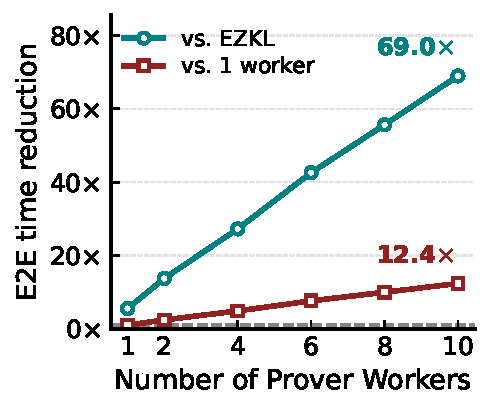
\includegraphics[width=\linewidth]{figures/new_eval/multi_node_scaling_NanoGPT_4L__time_reduction.pdf}
    \caption{NanoGPT (4L)}
    \label{fig:multi-nanogpt}
\end{subfigure}
\hfill
\begin{subfigure}[t]{0.32\textwidth}
    \centering
    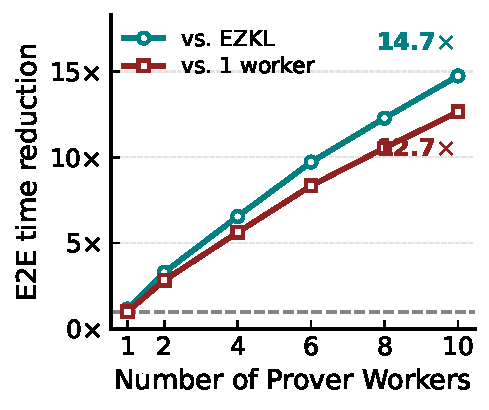
\includegraphics[width=\linewidth]{figures/new_eval/multi_node_scaling_MobileNet_time_reduction.pdf}
    \caption{MobileNetV2}
    \label{fig:multi-mobilenet}
\end{subfigure}
\hfill
\begin{subfigure}[t]{0.32\textwidth}
    \centering
    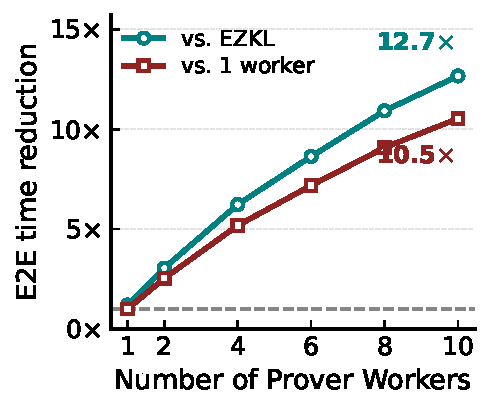
\includegraphics[width=\linewidth]{figures/new_eval/multi_node_scaling_BERT_Tiny_time_reduction.pdf}
    \caption{TinyBERT}
    \label{fig:multi-tinybert}
\end{subfigure}

\caption{
Multi-node scaling of \TITLE{} as prover workers are distributed across machines. 
Each plot reports speedup relative to the monolithic EZKL baseline and to \TITLE{} with one worker. 
Distributing workers across nodes reduces end-to-end request latency by increasing parallelism while avoiding the CPU and memory contention observed on a single machine.
}
\label{fig:parallel_multi_node}
\end{figure*}



\subsection{Scaling the Prover Worker Pool}
We next evaluate whether the schedulable jobs exposed by \TITLE{} can use additional cloud resources to reduce the latency of one proof-serving request. We vary the number and placement of prover workers and report end-to-end request time. We compare against both monolithic EZKL and the single-worker \TITLE{}+EZKL configuration. The first comparison captures the full benefit of changing the execution model, while the second isolates the incremental scaling obtained by adding worker capacity after partitioning.

\begin{figure}[t]
\centering
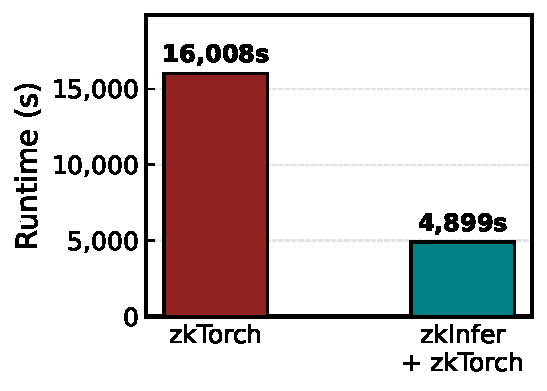
\includegraphics[width=0.75\linewidth]{figures/new_eval/1_zktorch_tinybert_runtime.pdf}
\caption{
Portability to zkTorch on TinyBERT. \TITLE{} executes partitioned proofs in parallel to reduce end-to-end proving time.
}
\label{fig:zktorch_tinybert}
\end{figure}

\subsubsection{\textbf{Parallel Execution on a Single Node}}

We first evaluate how much parallelism \TITLE{} can exploit within a single
machine. We vary the number of prover workers while keeping the hardware fixed
and measure warm end-to-end request latency.
Figure~\ref{fig:parallel_single_node} reports performance relative to both
monolithic EZKL and the single-worker \TITLE{}+EZKL configuration.

Increasing the number of prover workers reduces request latency for every
evaluated model. NanoGPT (4L) decreases from
\(\qty[quantity-product = {}]{1108}{\second}\) with one worker to
\(\qty[quantity-product = {}]{399}{\second}\) with 15 workers. This
corresponds to a \(\num{2.8}\times\) improvement over single-worker execution
and a \(\num{15.5}\times\) improvement over monolithic EZKL. MobileNetV2
decreases from \(\qty[quantity-product = {}]{9639}{\second}\) to
\(\qty[quantity-product = {}]{2384}{\second}\), a
\(\num{4.0}\times\) improvement over one worker, while TinyBERT decreases
from \(\qty[quantity-product = {}]{1022}{\second}\) to
\(\qty[quantity-product = {}]{333}{\second}\), a
\(\num{3.1}\times\) improvement.

% The benefit of additional workers diminishes at higher worker counts. Proving
% jobs vary substantially in runtime, so short jobs may finish while a small
% number of long-running jobs remain. At the same time, all prover workers on
% the machine share the same CPU and memory resources.
% Figure~\ref{fig:single-node-resource} illustrates this effect for MobileNetV2.
% As the number of workers increases, CPU and memory utilization approach
% saturation, leaving less additional capacity for each new worker and reducing
% the marginal improvement in request latency.



\subsubsection{\textbf{Parallel Execution Across Multiple Nodes}}

We next evaluate whether \TITLE{} can translate additional machines into lower
latency for a single inference request. We deploy one prover worker on each
m6a.4xlarge instance and vary the cluster size from one to ten nodes. Unlike
the single-node experiment, where all workers compete for the same CPU and
memory resources, each additional node contributes both a prover worker and
its own compute and memory capacity. Figure~\ref{fig:parallel_multi_node}
reports warm end-to-end request latency relative to monolithic EZKL and
single-worker \TITLE{}+EZKL.

Request latency decreases substantially as the cluster grows. For NanoGPT
(4L), increasing the deployment from one to ten workers reduces latency from
\(\qty[quantity-product = {}]{1108}{\second}\) to
\(\qty[quantity-product = {}]{89}{\second}\). MobileNetV2 and TinyBERT
exhibit similar improvements, reaching \(\num{12.7}\times\) and
\(\num{10.5}\times\) speedups over their single-worker executions,
respectively.

 
% The contrast with the single-node results is significant. Adding workers within one machine eventually yields diminishing returns because those workers share a fixed resource pool. Adding worker nodes instead increases the aggregate compute and memory available to the request. Fine-grained proving allows \TITLE{} to use this additional capacity by executing jobs concurrently across machines, extending latency reductions beyond the resource limits of a single node.

% These results show that the submodel graph exposed by \TITLE{} contains enough ready work to keep a distributed prover pool effective. The worker manager is able to dispatch submodel proofs across nodes without making orchestration the bottleneck, so request latency increasingly reflects the critical path through the partitioned computation rather than the cost of proving the full model on one machine. This is the main advantage of disaggregating proof generation: once the model is split into schedulable jobs, additional prover capacity can be applied to a single inference request.


% For NanoGPT (4L), multi-node execution provides the strongest scaling benefits. Runtime decreases from 1,108s with a single worker to 89s with 10 workers, corresponding to a 12.4$\times$ speedup relative to \TITLE{}'s single-worker configuration and a 69$\times$ speedup over the monolithic EZKL baseline. This improvement reflects both the large number of independent submodels and the ability to eliminate single-node memory and bandwidth bottlenecks through disaggregation. MobileNetV2 and TinyBERT also benefit significantly from multi-node parallelism. For MobileNetV2, runtime decreases from 9,639s to 762s as the number of workers increases from 1 to 10, yielding a 12.7$\times$ speedup relative to the single-worker configuration and a 14.7$\times$ speedup over EZKL. TinyBERT exhibits similar behavior, with runtime decreasing from 7,900s to 750s.



% \begin{figure}[t]
% \centering
% 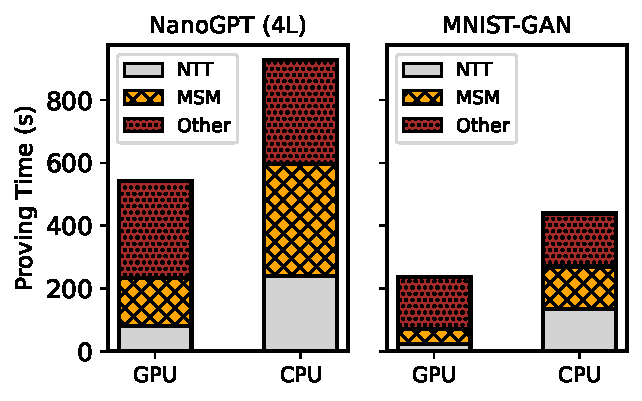
\includegraphics[width=\linewidth]{figures/evaluation/gpu_impact.pdf}
% \caption{
% Impact of GPU acceleration on Halo2 proof generation. 
% The figure breaks down proving time into NTT, MSM, and other components for NanoGPT (4L) and MNIST-GAN under CPU-only and GPU-accelerated execution. 
% GPU offloading reduces the dominant cryptographic operations, leading to lower end-to-end proof-generation time.
% }
% \label{fig:gpu_impact}
% \end{figure}

\subsection{Portability Across zkML Backends}
\label{subsec:extendingtoothersystems}

We evaluate \TITLE{} with zkTorch~\cite{chen2025zktorch} to test whether the execution layer generalizes beyond EZKL. zkTorch uses a different proving architecture, decomposing ONNX models into cryptographic basic blocks whose proofs are accumulated.
On TinyBERT, standalone zkTorch requires \(16{,}008\)~s on a single r6a.32xlarge instance. Using 15 prover workers, \TITLE{} reduces this to \num{4899}~s, a \(3.3\times\) improvement (Figure~\ref{fig:zktorch_tinybert}). This shows that \TITLE{} can accelerate a second zkML backend without modifying its core proving logic.



% \subsection{\textbf{GPU-Accelerated Proving}}
% \label{subsec:gpuhalo2}

% Finally, we evaluate whether GPU acceleration can further reduce the cost of proving the jobs created by \TITLE{}. For each model, \TITLE{} produces the same set of proving jobs, which are executed sequentially by a single prover worker. We compare two versions of this execution. The first uses CPU-only Halo2 proving, while the second offloads number-theoretic transforms (NTTs) and multi-scalar multiplications (MSMs) to an NVIDIA T4 GPU. All measurements run on an AWS g4dn.4xlarge instance with 16 vCPUs and 64~GB of memory. Since the proving jobs and execution strategy are identical in both cases, any difference in runtime comes from GPU acceleration within the Halo2 prover.

% Figure~\ref{fig:gpu_impact} shows that GPU acceleration reduces proof-generation time by \(1.7\times\) for NanoGPT (4L) and \(1.9\times\) for MNIST-GAN. Most of the reduction comes from faster NTT and MSM execution. These results show that GPU acceleration can further reduce the cost of each proving job and therefore complements \TITLE{}'s partitioned execution.